\documentclass[11pt, a4paper]{article}
\usepackage[a4paper, total={6.5 in,9in}]{geometry}
\usepackage[slovene]{babel}
\usepackage[utf8]{inputenc}
\usepackage[T1]{fontenc}
\usepackage{lmodern}
\usepackage{amsmath}
\usepackage{ amssymb }
\usepackage{amsfonts}
\usepackage{amsthm}
\usepackage{comment}
\usepackage{url}
\usepackage{gensymb}
\usepackage{subcaption}
\usepackage[pdftex]{graphicx}
\usepackage[section]{placeins}
\usepackage{mathtools}
\usepackage{float}
\usepackage{epstopdf}
\renewcommand{\vec}[1]{\mathbf{#1}}
\usepackage{hyperref}
\usepackage{wrapfig}
\usepackage{mhchem}
\pagestyle{plain}

\begin{document}

    \begin{center}
    {\LARGE\bfseries 6. Luščenje kemijskih parametrov\par}
    \vspace{1cm}
    
    {\Large Domača naloga pri predmetu Modelska analiza I\par}
    \vspace{0.2cm}
    {\normalsize Avtor: Matic Noč \par}
    \vspace{0.2cm}    
    {\normalsize 15.11.2017 \par}    

    
    \end{center}
\section{Uvod}
Obravnavali bomo problem "fitanja" oziroma luščenja parametrov linearnega modela - to je model, ki je linearen v neznanih parametrih $a_i$, kar pomeni da lahko luščimo parametre modelu s vsemi funkcijami, dokler je ta model linearna kombinacija neznanih koeficentov. Ne bi pa mogli npr. fitati $y = a_1 sin(x-a_2)$. Tak problem ima analitično rešitev s minimizacijo residualov oz. \textit{metodo najmanjših kvadratov - least squares}, ki pa nam ne da dober rezultat, če residuale ne obtežimo. 

\section{Odziv tkiva na reagente}

\subsection{Model}
Pri prvi nalogi smo obravnavali odziv tkiv na različne reagente, kjer gre za reakcijo, pri kateri spremljamo vezavo molekul reagenta $X$ na receptorje $Y$ v tkivu:
\begin{equation}
\ce{Y + X <=>Y^*}.
\end{equation}
V stacionarnem stanju tako dobimo zvezo
\begin{equation}
y=\frac{y_0x}{x+a},
\end{equation}
kjer pomeni $y_0$ nasičeni odziv tkiva in $a$ koncentracijo, potrebno za odziv, ki je enak polovici nasičenega. Enačbo lahko predelamo na linearni model tako da obrnemo enačbo (2)
\begin{equation}
\begin{split}
1/y &= \frac{1}{y0} + \frac{a}{y0x} \\
\widetilde{y} &= a_1\widetilde{x} + a_2 \\
\end{split}
\end{equation}
kjer je $\widetilde{y}=\frac{1}{y}$ in $\widetilde{x}=\frac{1}{x}$, $m=\frac{a}{y_0}$ in $n=\frac{1}{y_0}$. Pri tem se napake meritev $\sigma_y$ transformirajo $\sigma_{\widetilde{y}}$, dobimo pa jih lahko tako da odvajamo enačbo $\widetilde{y} = 1/y$.
\begin{equation}
\begin{split}
- 1/y^2 dy &=  d\widetilde{y} \\
\sigma_ {\widetilde{y}} &= \sigma_y \frac{1}{y^2}
\end{split}
\end{equation}

\subsection{Metoda najmanjših kvadratov}
Oglejmo si sedaj problem. Na voljo imamo tabelo podatkov $y_i,x_i$, ki smo jih npr. izmerili v laboratoriju. Transformirajmo podatke v $\widetilde{y_i}, \widetilde{x}_i$ in jih ustavimo v enačbo (3). Dobimo predoločen sistem enačb za koeficienta m,n
\begin{equation}
\widetilde{y_i} = m \widetilde{x}_i + n
\end{equation}
Ta sistem lahko zapišemo v matrični obliki
\begin{equation}
\vec{y} = X \vec{a}
\end{equation}
,kjer je 
\[
\vec{y} = 
	\begin{bmatrix}
	\widetilde{y_1}\\
	\vdotswithin{}		\\
	\widetilde{y_n}\\
	\end{bmatrix}.
\]
in 
\[
X=
  \begin{bmatrix}
    1 & \widetilde{x_1} \\
    \vdotswithin{...} & \vdotswithin{...}         \\
    1 &  \widetilde{x_n} \\
  \end{bmatrix}
\]
$\vec{a}$ pa je vektor neznanih koeficienotv
\[
\vec{a} = 
	\begin{bmatrix}
	a_1\\
    a_2 \\
	\end{bmatrix}.
\]
Rešitev poiščemo tako, da poiščemo take koeficiente $a_i$, ki minimizirajo kvadrat razlike napak med našim fitom in pravimi vrednostmi.
\begin{equation}
S = \sum (\widetilde{y_i} - f(x_i, a_1,a_2,...))^2
\end{equation}
Torej je naša najboljša rešitev za $a_i$ enaka rešitvi sistema enačb
\begin{equation}
\pmb{\frac{\partial S} {\partial a_i}  = 0 },
\forall i = 0,...,n_{meritev}
\end{equation}
Če zapišemo S v matrični obliki dobimo 
\begin{equation}
S = ||\vec{y}-X\vec{a}||^2
\end{equation}
Odvajamo po vektorju neznanih koeficientov in dobimo
\begin{equation}
\frac{dS}{d\vec{a}} = 2 (\vec{y} - X\vec{a}) X = 0
\end{equation}
oziroma matrični isti sistem enačb kot (8)
\begin{equation}
X^TX\vec{a} = X^Ty
\end{equation}
Torej rešitev $\vec{a}$ obstaja in je enaka
\begin{equation}
\vec{a} = (X^TX)^{-1} X^Ty
\end{equation}
Zaradi stabilnosti rešitev koeficiente ne dobimo s direktnim iskanjem inverza, ampak s reševanjem linearnega sistema enačb (11), ki ga lahko rešimo s LU, QR, SVD razcepom.
\subsection{Utežitev}
V osnovnem primeru, damo vsem točkam enako težo, kar seveda pomeni, da pri razpršenih podatkih ne bomo dobili dobrega fita, kot bomo kmalu videli. Utežimo zato residuale s  $\sigma_{y_i} =: \sigma_i$. Če je napaka velika, se na tiste točke ne oziramo močno, saj ne pripomorejo k večanju S, če pa je napaka majhna, pa je nujno da so točke fita in meritev blizu, saj bomo v nasprotnem primeru močno večali S.
\begin{equation}
S = \sum (\frac{\widetilde{y_i} - f(x_i, a_1,a_2,...)}{\sigma_i})^2
\end{equation}
Vidimo torej, da lahko naše podatke $\vec{y}$, $X$ le delimo s dano napako in uporabimo rešitev (12). \newline\newline 
Tako tudi $S$ postane pravi hi-kvadrat :  $S = \sum (\frac{y_i - y_{expected}}{\sigma})^2 = \chi^2$, kjer je $\chi^2$ porazdeljen po $N-M$ prostostnih stopenj. \newline\newline
Ko bo fit torej dober, mora biti naš $\chi^2$ blizu najbolj verjetnega, to je $N-M$, zato lahko definiramo reduciran $hi-kvadrat$ $\widetilde{\chi}^2 = \chi^2 /(N-M)$, ki mora biti pri dobrih parametrih enak 1 in je dobra mera za ugotavljanje dobrega fita.
\subsection{Varianca koeficientov $\vec{a}$}
Recimo da y ne poznamo točno in zapišemo naše izmerke kot $\vec{y' } = \vec{y} + \vec{\epsilon}$, kjer je $y$ prava vrednost in $\epsilon_i$ nekoreliran beli šum, porazdeljen okoli 0, $<\epsilon> = 0 $ z standardnim odklonom $<\epsilon_i \epsilon_j> = \sigma^2 \delta_{i,j}$. Torej je kovariančna matrika, v primeru enakih napak enaka $\epsilon^T\epsilon = \sigma^2 I$
 Naša rešitev v tem primeru ne bo točna ampak ocena $\vec{a'} = (X^T X)^{-1} X^T (y + \epsilon)$, kjer je $\vec{a'}$ ocena in $\vec{a}$ prava vrednost koeficientov. 
\begin{equation}
\vec{a'} = \vec{a} + (X^T)^{-1} X^T \epsilon
\end{equation}
Pričakovana vrednost ocene je kar enaka pričakovani vrednosti rešitve (11) $<\vec{a'}> = <\vec{a}>$, napaka koeficienotv pa bo varianca (koren povprčene vrednosti kvadrata napak) razlike ocene in in prave vrednosti.

\[
<(\vec{a'} - \vec{a})^2> = <(\vec{a'} - \vec{a})(\vec{a'} - \vec{a})^T> = <(X^TX)^{-1} X^T <\epsilon \epsilon^T >X (X^TX)^{-1}  \epsilon>
\],
kar je v primeru, ko je $<\epsilon \epsilon^T > = \sigma^2 I $ enako kar 
\begin{equation}
var (\vec{a}) = M = \sigma^2(X^TX)^{-1}
\end{equation} 
Če napak meritev ne poznamo, potem lahko ocenimo napako kota reduciran $\widetilde{\chi}^2 = \frac{\chi^2}{N-M}$, če pa uporabljamo uteži iz ocene napak pa 

\begin{equation}
M=X^{\rm {T}}WX)^{-1}X^{\rm {T}}WMW^{\rm {T}}X(X^{\rm {T}}W^{\rm {T}}X)^{-1} 
\end{equation} 
Če so naše uteži kar napake $W = M^{-1}$:
\begin{equation}
M=(X^{\rm {T}}WX)^{-1}
\end{equation}
Torej v primeru ko so naše uteži napake lahko le izračunamo inverz matrike $(X^{\rm {T}}WX)^{-1}$
\subsection{Reševanje brez upoštevanja napak}
Podatke sem obrnil in na matriki $X$ uporabil metodo $np.linalg.lstsq$, ki uporabi SVD razcep za najhitrejši izračun rešitve sistema (11)
\begin{figure}[H]
\hspace*{-2.2cm}     
  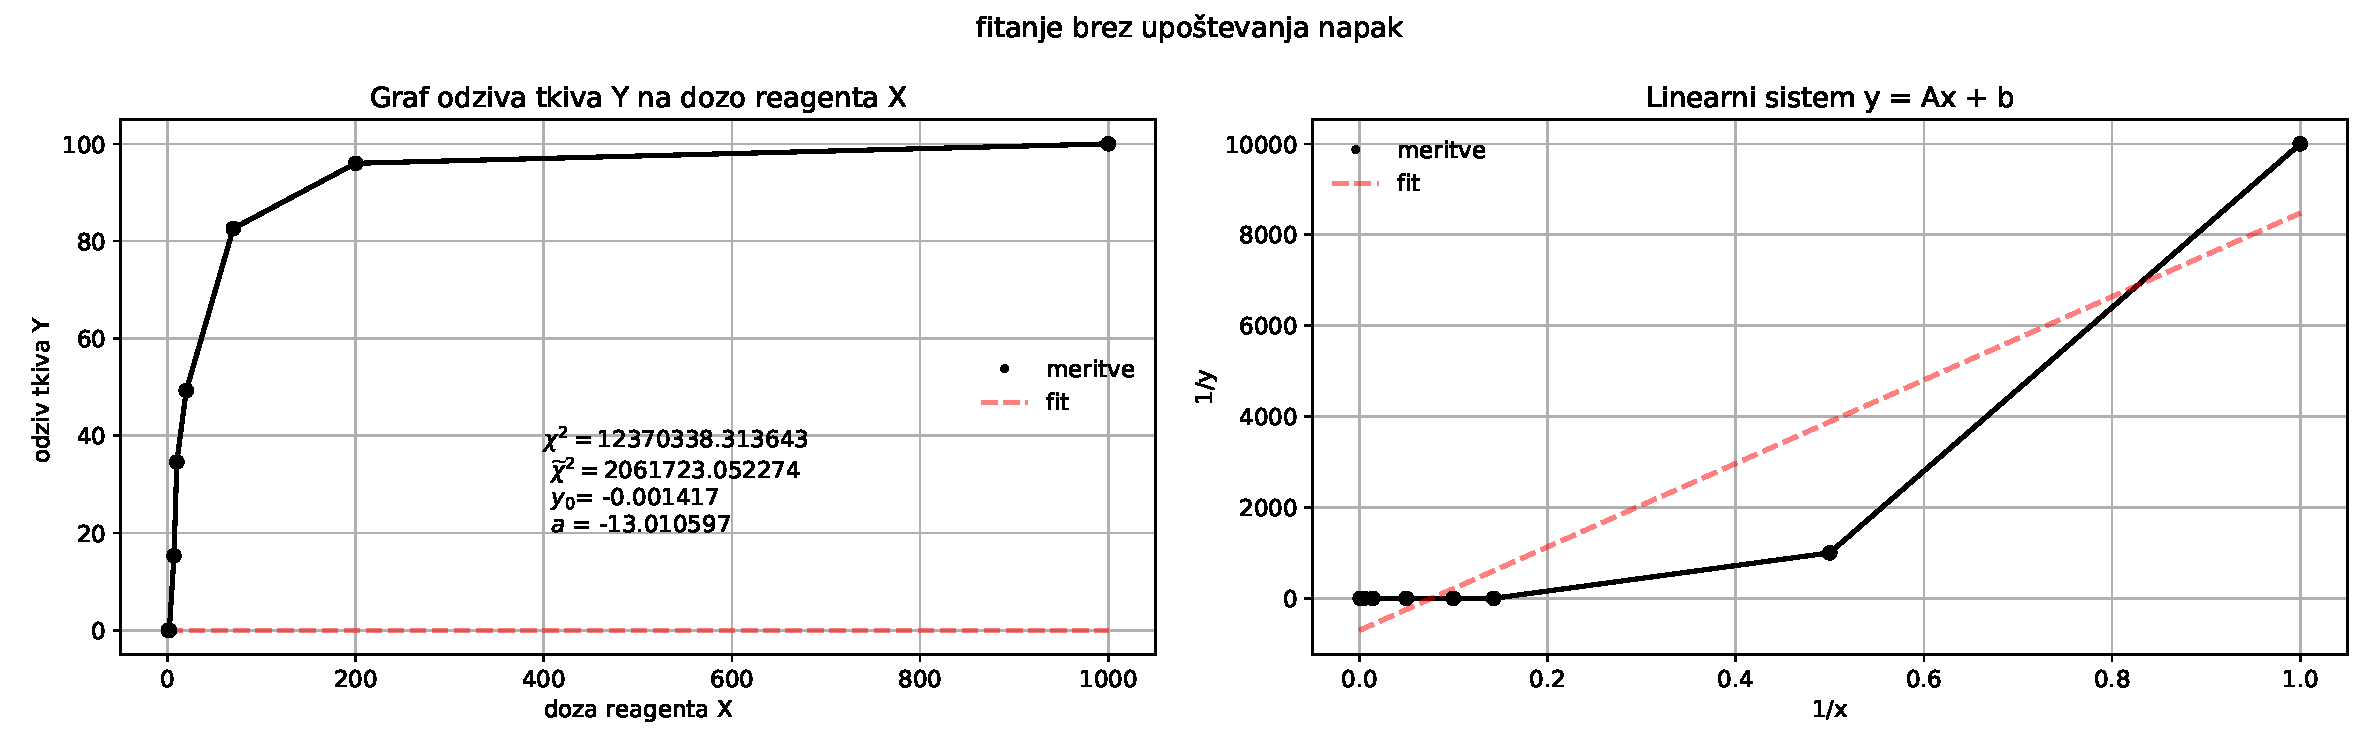
\includegraphics[width=20.5cm]{prva_brez_napak.pdf}  
\end{figure}
Že na grafu vidimo, da so ti parametri napačni, kar nam pove tudi vrednost $\widetilde{\chi}^2$. Ker ni utežitve morajo parametri vsem točkam zagotoviti enako dobro bližino, kar pomeni, da se ne skoncentrira na točke s majhno napako. 

\subsection{Reševanje s napakami}
\[
X=
  \begin{bmatrix}
    \frac{1}{\widetilde{\sigma}} & \frac{\widetilde{x}}{\widetilde{\sigma}} \\
    \vdotswithin{...} & \vdotswithin{...}         \\
    \frac{1}{\widetilde{\sigma}} & \frac{\widetilde{x}}{\widetilde{\sigma}} \\
  \end{bmatrix}
\]
in 
\[
\vec{y} = 
	\begin{bmatrix}
	\frac{\widetilde{y}}{\widetilde{\sigma}}\\
	\vdotswithin{}		\\
	\frac{\widetilde{y}}{\widetilde{\sigma}}\\
	\end{bmatrix}.
\]
Za varianco napak sem še vedno sem dobiti inverz matrike $(X^TWX)$, ki sem ga dobil s metodo $np.linalg.inv$. Tako sem dobil tudi korelacijske koeficiente in napake parametrov.
\begin{figure}[H]
\hspace*{-2.8cm}     
  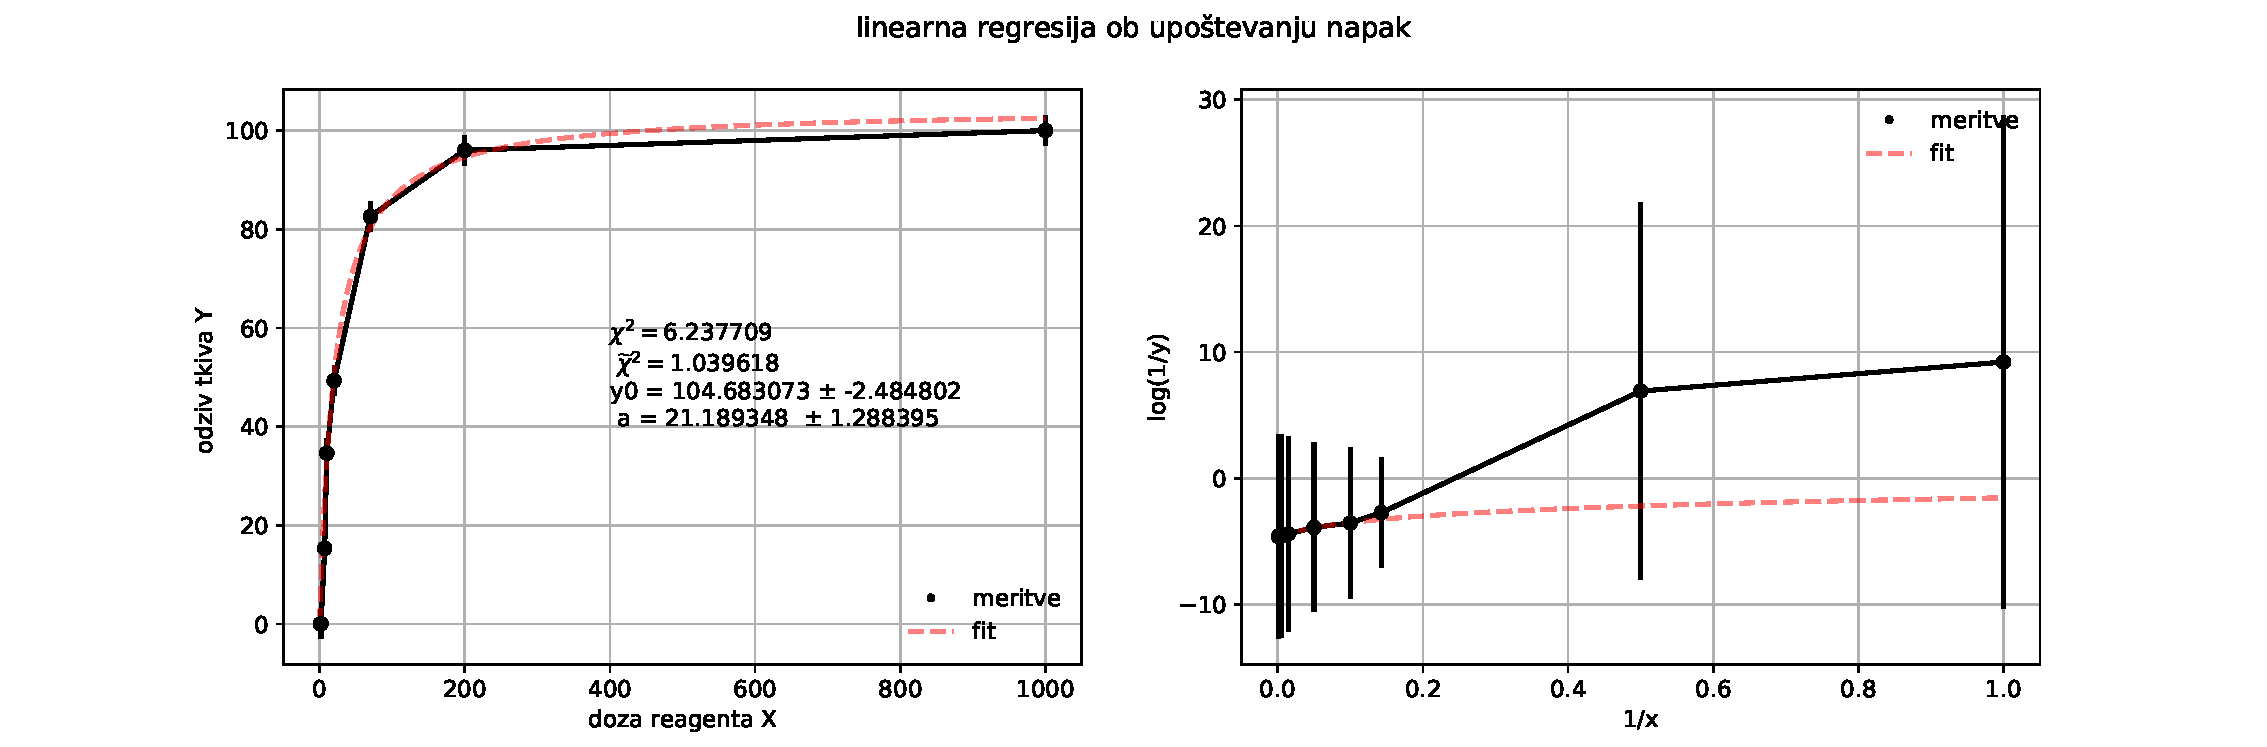
\includegraphics[width=23cm]{prva_upostevanje_napak.pdf}
 
\end{figure}
Vidimo, da tokrat je rešitev veliko bolj pravilna, saj je točke, ki imajo veliko napako zaradi utežitve lahko izpustil (desni graf je prikazan v logaritemski skali!), $\widetilde{\chi}^2$ pa je zelo blizu 1, kar pomeni, da je zelo malo verjetno, da naš fit ni pravi in je posledica statističnega naključja.
\section{Visokoločljivostni magnetni spektrometer}
Ko delce spustimo skoz magnetno polje, se njihov tir ukrivi. Če izmerimo kje se nahajajo na detektorju, lahko napovemo kje so se nahajali delci na tarči, in iz katere smeri so (pri)leteli, 
iz tega pa njihove energije in kinematske količine.\newline
Torej imamo dva seta koordinat $(x_{tg},y_{tg},\theta_{tg},\phi_{tg})$ in v goriščni ravnini detektorja: $(x_{fp},y_{fp},theta_{fp},\phi_{fp})$, kjer so x,y položaj trka na detektorju in $\phi,\theta$ azimutalni in zenitni kot trajektorje. V splošnem je vsaka koordinata na tarči kombinacija vseh ostalih, zato se bomo posvetili le eni od tarčevskih koordinat $\theta_{tg}$. Izmerjeni kalibracijski podatki so $x_{fp}, \phi_{fp}$ torej iščemo preslikavo
\begin{equation}
(x_{fp}, \phi_{fp}) => \theta_{tg}
\end{equation}
Vzeli bomo nekaj različnih preslikav in skušali najti tako, ki nam bo dala $\widetilde{\chi}^2 \sim 1 $. Najprej se prepričajmo da nam podatki ne prikažejo ničesar, saj jih lahko plotamo na 3D grafu
\begin{figure}[H]
\hspace*{-2cm}     
  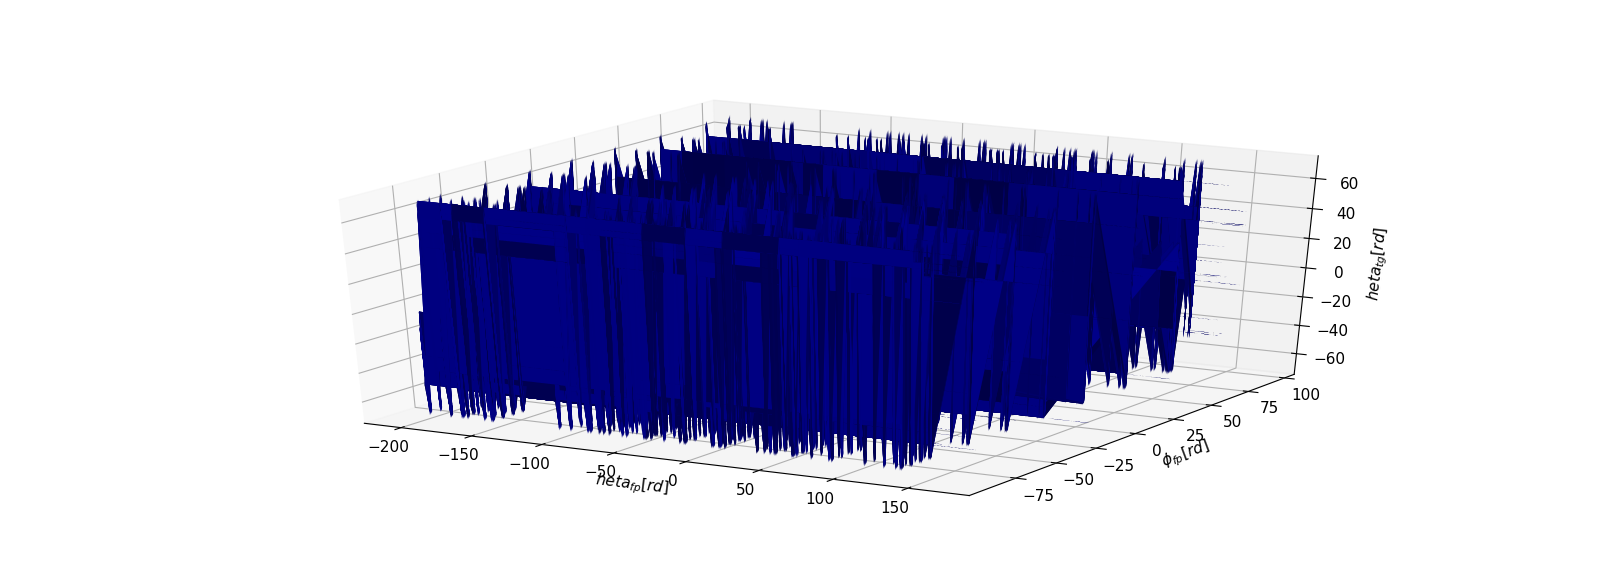
\includegraphics[width=15cm]{aa.png}
  \caption{iz podatkov ne vidimo nič} 
\end{figure}
\subsection{Linearni model}
Vzemimo najprej naiven linearni model 
\begin{equation}
\theta_{tg} = a_0 + a_1 \theta_{fp} + a_2 x_{fp}
\end{equation}
Pričakujemo, da ni linearne ravnine, ki nam dobro opisala zgornjo sliko.
\begin{table}[H]
\centering
\caption{Linearni testni model}
\label{my-label}
\begin{tabular}{lll}
	$\widetilde{\chi}^2$ & 354.488
&  \\
 $a_0$ & -6.642701150896979101e+00 $\pm$ 0.0026895426110164398&   \\
 $a_1$ & -8.402619006911082877e-01 $\pm$ 5.2782693856238785e-05&  \\
 $a_2$ & 9.736583733416463993e-01 $\pm$7.22595806240393e-05   , 
\end{tabular}
\end{table}
Tako kot smo pričakovali tak fit nima smisla
\subsection{Izboljšava modela}
Vzemimo, da je naša ravnina lahko ukrivljena in tako začnimo s dodatnimi kvadratnimi potencami, napak fita zaradi preglednost in ne bistvenosti ne bom več pisal

\begin{equation}
\theta_{tg} = a_0 + a_1 \theta_{fp} + a_2 x_{fp} + a_3 x_{fp}^2 + a_4 \theta_{fp}^2
\end{equation}

\begin{table}[H]
\centering
\caption{Kvadratni model}
\label{my-label}
\begin{tabular}{lll}
	$\widetilde{\chi}^2$ &8.11274154
&  \\
 $a_0$ & 1.05023609151 \\
 $a_1$ &  -0.849920201119   \\
 $a_2$ &  -2.93380021016e-05  \\
 $a_3$ &   0.985348592305 \\
 $a_4$ & -0.00180972046672,
\end{tabular}
\end{table}
Vidimo, da se je fit bistveno izboljšal vendar je še vedno daleč od 1.\newline\newline
Vzemimo še višje potence, mešane člene.
\begin{equation}
\theta_{tg} = a_0 + a_1 \theta_{fp} + a_2 x_{fp} + a_3 x_{fp}^2 + a_4 \theta_{fp}^2 +a_5  x_fp\theta_{fp} + a_6 x_{fp}^2\theta_{fp}+ a_7 x_{fp}\theta_{fp}^2
\end{equation}

\begin{table}[H]
\centering
\caption{Višje potence}
\label{my-label}
\begin{tabular}{lll}
   
     
	$\widetilde{\chi}^2$ &2.50906764
&  \\
 $a_0$ &  1.68357878e+00\\
 $a_1$ &   -8.50988358e-01    \\
 $a_2$ &  -2.66485613e-04   \\
 $a_3$ &    9.79401322e-01 \\
 $a_4$ & -2.14775172e-03 \\
 $a_5$ &  5.47218368e-04   \\
 $a_6$ & 4.01308547e-06  \\ 
 $a_7$ &  -2.02687574e-06 ,
\end{tabular}
\end{table}
$\widetilde{\chi}^2$  se še zmanjša vendar pa višje potence ne bodo nikoli dobro fitale problema, saj potenčne funkcije med seboj niso ortogonalne in ne bodo pokrile vseh možnosti. Smisleno bi bilo poskusiti s ortogonalnimi funkcijami 
npr
\begin{equation}
\theta_{tg} = \sum a_n sin(nx_{fp})+ \sum b_n cos(n\theta_{fp}))
\end{equation}
 kjer vzamemo visoko število $n$, toda ti ne dajo dobre rešitve, saj sem se s 300 sinisi približal šele $\widetilde{\chi}^2 = 1.277904083153612591e+00$. Vseeno pa je bil to najboljši fit.\newline



\section{Absorbcijski spekter Kadmija v okolici različnih kemijskih elementov}
V tej nalogi smo želili preučiti abosrbcijski spekter Kadmija v rastlinah. Vemo, da je absorbcijski spekter Kadmija odvisen od elementov, ki so v okolici, vendar teoretično še ne znamo dobiti pravo odvisnost, zato si pomagamo s luščenjem parametrov, saj vemo, da je spekter linearna kombinacija dveh spektrov, ko je Kadmij okolici sulfata in vezan na žveplo in ko je v okolici pektina in vezan na kisik. Ta predpostavka pomeni, da se v rastlinah pretežno veže le na te dva elementa. \newline\newline
\begin{figure}[H]
\hspace*{-2.2cm}     
  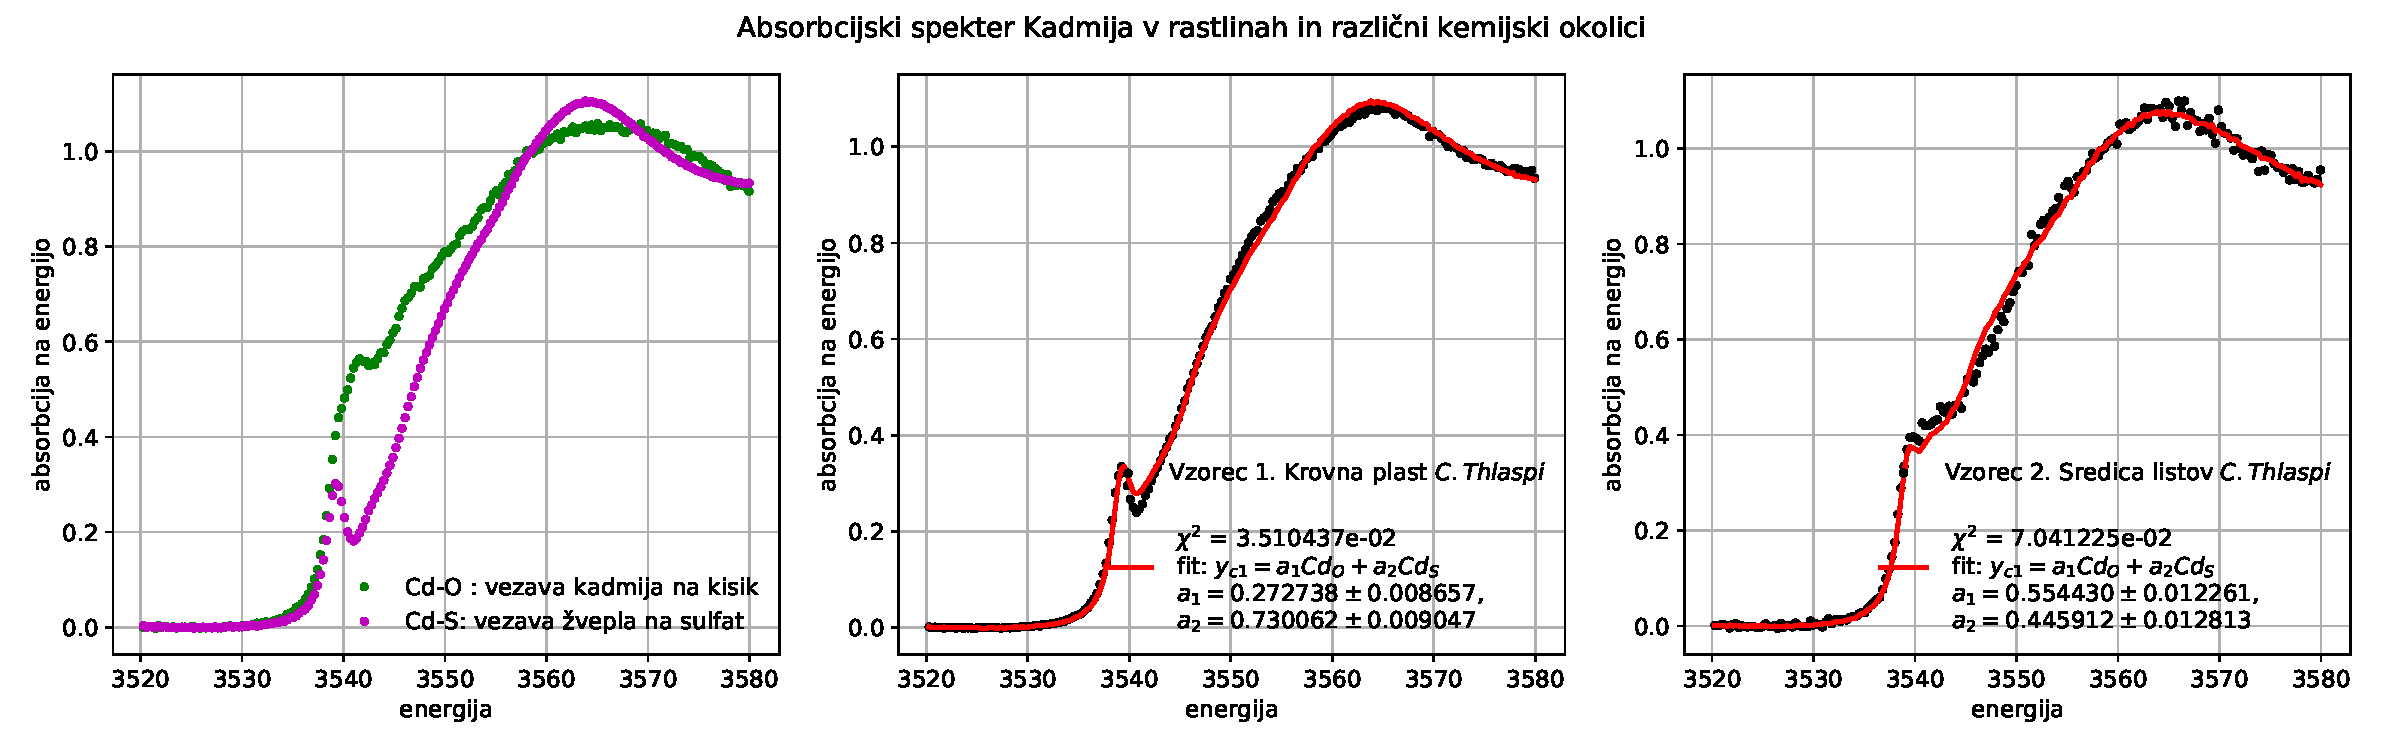
\includegraphics[width=20.5cm]{tretja_fit.pdf}
  \caption{Levo: absorbcijska spektra Kadmija ob različnih vezavah elementov, desno: izmerjen absorbcijski spekter krovne plasti in sredice listov. Opazimo več stvari: 1)fit je na oko kar dober, čeprav se zdi da smo naleteli na $"overfit"$, torej popolno prileganje podatkom, pa je to le posledica, da nismo obtežili problema s napakam, ki so majhne, saj so majhni tudi podatki. 
  2) v krovni plasti je več kadmija vezanega na žveplo, torej je v okolici več sulfata z glutationom, medtem ko je v listni sredici malce več kadmija vezanega na kisik.
  Za variančno matriko sem potreboval napako, za katero sem vzel kar $\widetilde{\chi}^2$.}
\end{figure}
Realno vrednost $\chi^2$ bi dobili, če bi podali neko oceno za napake. Tu je nujno da so vse napake enake, ker nam enakomerna utežitev da dober rezultat. Glede na to da želimo imeti $\widetilde{\chi}^2 \sim 1 $, lahko obratno ocenimo napake tako da izračunamo $\sigma^2 = \frac{\chi^2}{N-M}$, saj je $\chi^2 \sim N-M$, ko je fit dober (vidimo iz slike). Torej je naša napaka $\sigma_1 = 0.013$ in $\sigma_2 = 0.018$. Ker je utežitev enakomerna vpliva le na vrednost $\chi^2$ in ne na obliko grafa.
\begin{figure}[H]
\hspace*{-2cm}     
  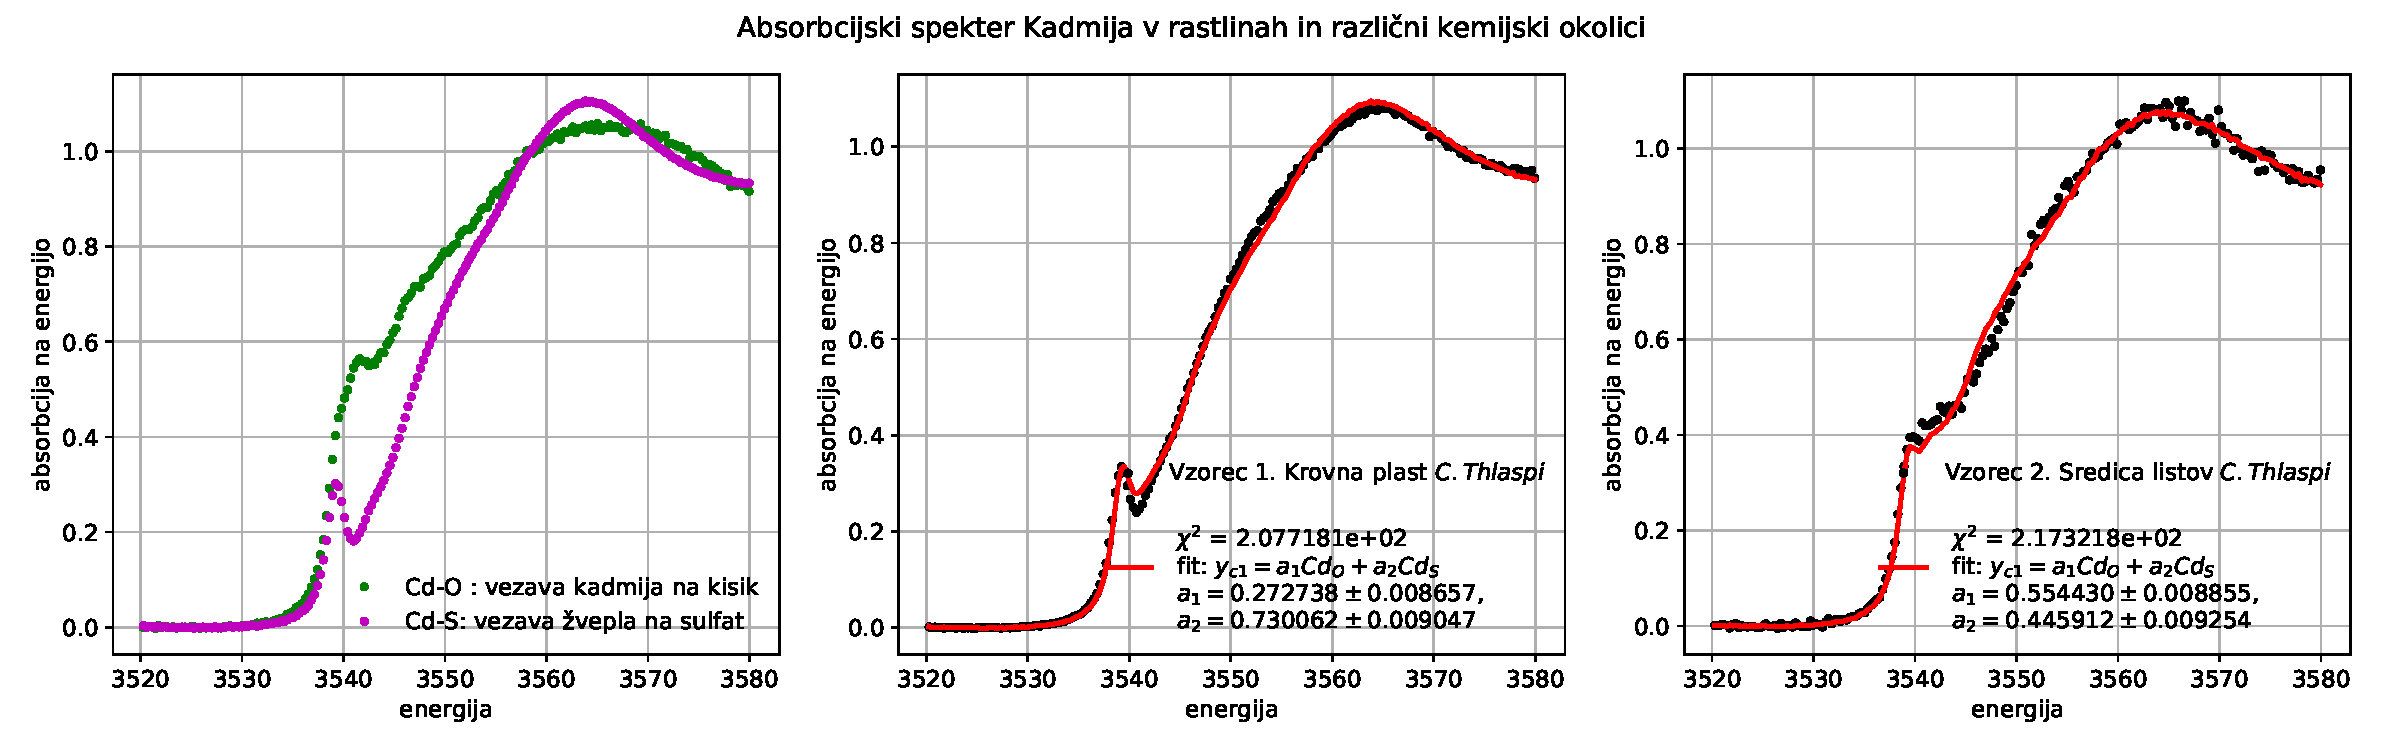
\includegraphics[width=20cm]{tretja_fit_brez_vpliva.pdf}
  \caption{Vidimo, da napaka le zveča $\chi^2 \sim 200 = N-M$} 
\end{figure}




\section{Zaključek}
Naučili smo se luščiti linearne parmetre in ocenjevati kako dober fit je, saj vidimo, da v več dimenzionalnem prostoru ne moremo kar na grafu videti ali je fit dober. Dobro bi bilo implementirati neke vrste strojno učenje, kjer bi avtomatizirali postopek; torej bi model sam dodajal različne parametre in na testnih podatkih iskal najboljši fit, ter se tako $"naučil"$ najboljše preslikave. Zaradi velikega števila podatkov, nikjer nismo opazili "overfita", ko vzameš preveč parametrov in začne $\chi^2$ zaradi tega močno padati. Videli smo da je ocena napak zelo pomembna, saj nam da veliko informacij o tem katere točke so najbolj pomembne.

\end{document}